\section{轮轴}\label{sec:7-4}

利用桔槔从井中提水,井中水面必须离井口相当近,因为桔槔能够转动的角度不大,水桶提升的高度也不能很大。
所以要从深井中提水,桔槔这样简单的杠杆就无能为力了。
如果我们能够造出象图 \ref{fig:7-15} 那样的可以连续旋转的杠杆,使动力臂、阻力臂都连续绕支点 $O$ 旋转,
让被提起的绳子绕在随着旋转的圆筒上,水桶提升的高度就可以大大增加。
辘轳(图 \ref{fig:7-16})就是这样的杠杆。

\begin{figure}[htbp]
    \centering
    \begin{minipage}{5cm}
    \centering
    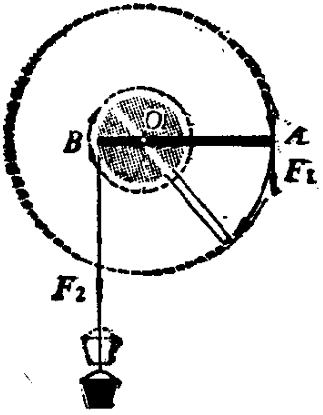
\includegraphics[width=4cm]{../pic/czwl1-ch7-15}
    \caption{}\label{fig:7-15}
    \end{minipage}
    \qquad
    \begin{minipage}{9cm}
    \centering
    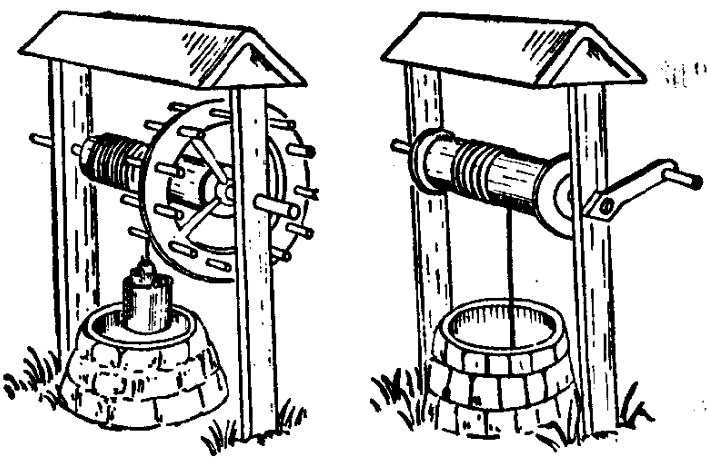
\includegraphics[width=8cm]{../pic/czwl1-ch7-16}
    \caption{辘轳}\label{fig:7-16}
    \end{minipage}
\end{figure}

辘轳是由一个木轴和一个大轮构成的(通常也用摇臂代替大轮),木轴和大轮的轴线相合,
辘轳的轮半径或摇臂就是图 \ref{fig:7-15} 中杠杆的动力臂 $OA$。
辘轳的轴半径就是图 \ref{fig:7-15} 中杠杆的阻力臂 $OB$,
辘轳的轴心就是图 \ref{fig:7-15} 中杠杆的支点 $O$。
象辘轳这类由轮和轴组成,能绕共同轴线旋转的简单机械,叫做\textbf{轮轴}。
\CJKunderwave{轮轴实质是可以连续旋转的杠杆}。

根据杠杆平衡条件和图 \ref{fig:7-15} 可以知道
$$ F_1 \cdot OA = F_2 \cdot OB \quad \text{或} \quad \dfrac{F_2}{F_1} = \dfrac{OA}{OB} \;\juhao $$

如果轮半径用 $R$ 表示,轴半径用 $r$ 表示,上式可以写成
$$ \dfrac{F_2}{F_1} = \dfrac{R}{r} \;\juhao $$

所以,\CJKunderwave{轮半径是轴半径的几倍,作用在轮上的动力 $F_1$ 就是作用在轴上的阻力 $F_2$ 的几分之一}。
可见,使用轮轴可以省力。想想看,这时动力的作用点是少移动了距离还是多移动了距离?

轮轴的应用很广,除辘轳以外,汽车驾驶盘(图 \ref{fig:7-17}),厂矿里用的手摇卷扬机(图 \ref{fig:7-18}),都是轮轴的实例。

\begin{figure}[htbp]
    \centering
    \begin{minipage}{7cm}
    \centering
    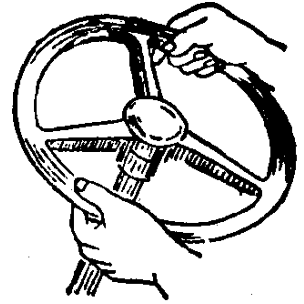
\includegraphics[width=4cm]{../pic/czwl1-ch7-17}
    \caption{汽车驾驶盘}\label{fig:7-17}
    \end{minipage}
    \qquad
    \begin{minipage}{7cm}
    \centering
    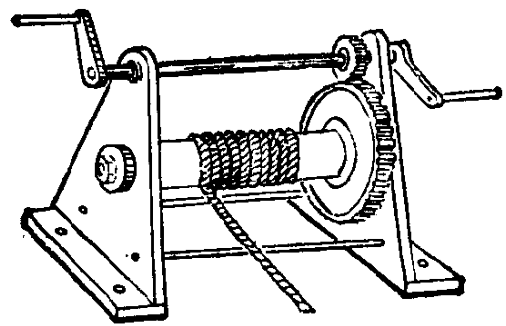
\includegraphics[width=7cm]{../pic/czwl1-ch7-18}
    \caption{手摇卷扬机}\label{fig:7-18}
    \end{minipage}
\end{figure}



\lianxi

(1) 拧螺丝用的扳手(图 \ref{fig:2-13})是个轮轴。手握在扳手柄的末端拧螺丝,比握在柄的中部省力,为什么?

(2) 用螺丝刀拧螺丝钉的候,手握在螺丝刀杆上和握在螺丝刀柄上一样费力吗?为什么?

(3) 使用轮轴的时候,如果动力作用在轴上,阻力作用在轮上,是省力还是费力?是少移动距离还是多移动距离?为什么?

(4) 观察一辆自行车,指出它的哪些装置是杠杆,哪些装置是轮轴。

